\documentclass[10pt,a4paper,twocolumn]{article}
\usepackage[cm]{fullpage}
\usepackage{newtxtext}
\usepackage{newtxmath}
\usepackage{outlines}

\usepackage{graphicx} %插入图片的宏包
\usepackage{float} %设置图片浮动位置的宏包
\usepackage{subfigure} %插入多图时用子图显示的宏包

\usepackage{xcolor}
\definecolor{light-gray}{gray}{0.95}
\newcommand{\code}[1]{\colorbox{light-gray}{\texttt{#1}}}

\usepackage{listings, listings-rust}
\usepackage{xparse}

\lstset{language=Rust,keywordstyle={\bfseries \color{blue}}}

\begin{document}

\title{Advanced Systems Programming (H) 2021-2022 – Exercise 1}
\author{Yao Du, 2359451D}
\date{\today}

\maketitle 

\section*{Part 1}

% you should research and prepare a description of how memory management works in the Rust programming language, and how the Rust language manages ownership of data, including different pointer types and borrowed references to data. You should describe when memory allocations occur in Rust programs, how Rust tracks ownership and borrowing of data, and when it deallocates memory. [10 marks] 你应该研究并准备描述内存管理在Rust编程语言中是如何工作的,以及Rust语言如何管理数据的所有权,包括不同的指针类型和借用数据的引用。你应该描述Rust程序中何时发生内存分配,Rust如何跟踪数据的所有权和借用,以及何时取消内存分配。[10分]

% \1 内存管理在Rust编程语言中是如何工作的
% \1 Rust如何管理数据所有权
    % \2 不同指针类型, 借用数据的引用
    
% \1 Rust何时发生内存分配
% \1 Rust如何跟踪数据所有权,和引用租借
% \1 Rust如何回收内存分配

% 内存管理在Rust编程语言中是如何工作的
There are several typical approaches of memory management, which can be categorized into two main kinds: manual and automatic memory management. Languages, for example, C requires programmer to manage the memory and resources manually but error-prone. JVM-based Languages like Java, Scala use garbage collectors which releases the heap space automatically, however, requires more runtime overheads. Specifically, many scripting languages (Python, Ruby) adopt an automatic management model called reference counting. It is surely predictable and understandable, but requires extra space to store the references. And it is not suitable for low-level code where performance is critical-concerned. Specifically, the automatic memory management of Rust is based on an approach of region-based lifetime tracking, offering more predictability and stronger compile-time behavior guarantees. 

The region-based model is derived from the concept of stacked-based memory management. Every function call would push a new frame onto the stack, holding corresponding local variables and parameters. When current function finished, the frame with the contents would be then popped out from the stack. The scopes of functions are usually nested within the other, and the lifetime of the content stored on them is based on the scope of that frame. It can be assumed that every construct has its own scopes/regions. And every variable lives within a region, and is automatically allocated when entering that region, and deallocated when leaving that scope. Rust extends this model to manage the heap, tieing object lifetimes to stack frames. Allocate objects with lifetimes corresponding to regions. Also, track how objects are passed between stack frames i.e. ownership tracking. While the object has been passed to other regions, deallocating objects only when the lifetime of their owning region ends. And this is achieved by the destructor for the type i.e. \code{drop()} method is called. 

The code snippet below shows an example of the smart pointer \lstinline[language=Rust]{Box<T>} which allows to store a value on the heap and returned a local variable \code{b} on the stack, pointing to the allocated heap memory. The lifetime of \code{b} is based of the stack frame it resides. The heap allocated object has lifetime matching that of the Box. So when \code{b} goes out of scope, its destructor is automatically called by the compiler and the corresponding heap memory is freed as well.
\begin{lstlisting}[language=Rust, style=boxed, caption={Using Box<T> to Point to Data on the Heap}]
fn main(){
    let b = Box::new(5);
    println!("b={}", b);
} // here b and the heap memory 
// it points to would be deallocated
\end{lstlisting}

The key difference between Rust and other programming languages and the core of region-based memory management is the ownership tracking. And the ownership is a set of rules that governs how to manage Rust program memory. Also, it is requires that Rust compiler and type system tracks ownership (borrow checker) of all data in a program. The Rust compiler should know when a value has been consumed, when it’s reached the end of its lifetime.

And there are three ownership rules:
\begin{outline}
    \1 Every value in the program has a single owner at all times
    \1 There can only be one owner at a time
    \1 When the owner goes out of scope, the value should be dropped
\end{outline}

Rust also defines rules about the transfer of ownership of data in function and method calls. The first case (Listing 2) is that, a function which passed a parameter by value would take ownership of that value. It can be seen that the string variable \code{s1} is passed to the function \lstinline{fn takes_ownership}, i.e. the ownership would be taken. So if we attempt to copy the pointer, length, and the capacity of the String data that are on stack and assigns it to \code{s2} (namely, moves \code{s1} into \code{s2}) at the line 4, a compile time error is reported. Because Rust considers \code{s1} as no longer valid. This actually avoids the double free error where both \code{s1} and \code{s2} go out of scope, they will both try to free the same memory. And at this example, the memory which \code{s1} points to would be deallocated by the function \lstinline{fn takes_ownership} and \code{s2} would never get a chance to free up the same memory in main().

\begin{lstlisting}[language=Rust, style=boxed, caption={Ownership Move and Stacked-based Value Copy}]
fn main(){
    let s1 = String::from("hello");
    takes_ownership(s1);
    let s2 = s1; // Error, 
    //the ownership of s1 is moved

    let x =5;
    makes_copy(x); // x(primitives)
    // is copied into func
    // and x is still valid
}

fn takes_ownership(some_string: String){
    println!("{}", some_string);
}// drop some_string when ends

fn makes_copy(some_integer: i32){
    println!("{}", some_integer);
}// drop value copy here
\end{lstlisting}

It is also noticeable in Listing 2 that, for types which implements the \code{Copy} trait, Rust would perform value copy. Some simple types already implement it since this is cheap computationally. So we can still use the variable \code{x} after line \code{8}, as \code{x} itself is still valid in main(). 

In Rust, a function can give ownership of a value to its caller, making the caller responsible for freeing that resource. The function or method cannot retain any references to the resource when it gives up ownership in this way. (Listing 3)

\begin{lstlisting}[language=Rust, style=boxed, caption={Function Return Ownership}]
fn main(){
    // get the ownership from function
    let s1 = give_ownership();
} // main is responsible 
// to deallocate s1

fn gives_ownership() -> String{
    let some_str = String::from("hello");
    // return the ownership of some_str 
    // to caller
    some_str
}
\end{lstlisting}

In some cases, we just want to use value in function rather than get the ownership of that value, we need the concepts of borrowing reference. When a parameter is borrowed, ownership of the resource remains with the caller. The function can use the resource it’s borrowed for the duration of the call, but no longer. And when the function returns, the caller still has access to and ownership of the resource. In default case, the borrowing reference defined by \lstinline{&} symbol is immutable.

Listing 4 shows the default immutable reference of \code{s1} is passed to \lstinline{fn calc_len}. And when \code{s} of \lstinline{fn calc_len} goes out the scope, nothing happens as it is a reference to a String and does not have ownership of what it refers to. Additionally, we are not allowed to change the borrowed value in this case.
\begin{lstlisting}[language=Rust, style=boxed, caption={Borrowing Reference}]
fn main(){
    let s1 = String::from("hello");

    let len = calc_len(&s1);//borrow

    println!("len is {}", len);
}

fn calc_len(s: &String) -> usize{
    // Error, cannot change the value 
    // via immutable reference
    // s.push_str(", world"),
    s.len()
}
\end{lstlisting}

In contrast to immutable reference, Rust provides the unique reference to mutable object which is labeled by \lstinline{&mut}. And to change an object, we either own the object which is not marked as immutable or own the unique \lstinline{&mut} reference to it. Distinguish with these two different references, we can avoid the data races and iterator invalidation in Rust, as the Rust compiler and runtime system work together to control how references can be used, and to track ownership of references and the referenced values. The restriction are:
\begin{outline}
    \1 An object of type T can be referenced by multiple immutable references. Or it can be referenced by exactly one mutable reference
    \1 It is not allowed to have both mutable and immutable references to the same object simultaneously
    \1 An immutable object cannot be referenced as mutable
    \1 A mutable object can be referenced as immutable which would make this object immutable during the referenced time
\end{outline}
As the elements of iterators in Rust are immutable references, it guarantees that the element cannot be changed. Meanwhile, no mutable references to the object can exist in compile time. Thus, iterator invalidation problem could be detected.

This restriction however make it impossible to express certain cyclic data structures in Rust, e.g. doubly linked-list. It trades expressive power for safety. Luckily, Rust also has a third type of reference, known as the raw pointer (\lstinline{*const T} and \lstinline{*mut T}) which works just like C pointers. And by using it, it is possible to write cyclic data structures in the same way as C, but is exposed to memory safety issues. Programmer effort is needed to manage it manually as raw pointers have no automatic clean-up and are not guaranteed to point to valid memory. 

It is worth mentioning that, reference in Rust has its own lifetimes (except for raw pointers), which is the scope for which that reference is valid. And if the lifetime is not annotated explicitly, Rust has implicit rules to infer the lifetimes in general cases. This technique provides compiler with enough information to prevent us from unsafe memory behavior like dangling pointer.  

\section*{Part 2}

C takes stacked-based approach to manage the stack automatically which is effective. And the pattern of region-based memory management is derived from it, so both Rust and C can effectively manage the stack. However, C requires programmer to manage the heap memory manually. Using \code{malloc()} to allocate the heap memory and \code{free()} to free up the space. So it is common that memory leaks exist in C program if things related to heap are not processed successfully, and usually C compilers do not provide any approaches to report these errors before running the code. Once errors exist, it is hard to debug the root cause, especially in data races case. Also, managing memory manually has unpredictable overheads. As a programmer we have no idea how long those calls will take to execute. By contrast, Rust has the concepts of ownership tracking and lifetimes, enforcing many unsafe runtime behaviors to be checked efficiently in compile time. The data is clean-up automatically at the end of their lifetime when goes out of scope without the explicit syntax. And it offers predictable timing and has no run-time cost compared to manual heap memory management. Though, it loses generality, since the region-based management pattern ties the lifetime of heap allocation to that of stack frames.

Since C requires extra effort to manage the heap, there are several runtime bugs might happen: use-after-free, double free, iterator invalidation and race conditions. Type system of Rust tracks ownership and each value can only have one owner at the same scope so use-after-free or double free problems can be prevented at the compile time. The destructor of data would be called safely when it goes out of the scope which holds the ownership. As for data races with multiple threads, the restriction on how to use the borrowing references make it impossible for two threads to each have a mutable reference to the same object. As mutable and immutable reference to a mutable object cannot exist in the same scope simultaneously. It further prevents the iterator invalidation as the iterator in Rust requires the immutable reference of the object. So it is impossible to change the object being iterated over whilst the iterator exists. No dangling reference exists in Rust, as the borrow checker would check and infer the lifetimes of references. So any invalid reference will be detected before crashing at runtime.  Consider that Rust compiler generates exactly the same code to allocate and free memory at the correct places as an equivalent C program using malloc and free. Consequentially, the timing and memory usage of Rust code is predictable.

However, the restriction rules about ownership and borrowing make it also impossible to express cyclic data structures in Rust safely. So at this point, programmer needs to use the raw pointer just like in C with care. Moreover, Rust cannot express shared ownership of mutable data while multiple references to point to immutable an object is fine. Because the shared ownership of mutable data might lead to race conditions. But Rust still provides the \code{RefCell} type, allows callers to borrow or mutably borrow the wrapped value, and enforces at run time that there can only be immutable borrows or a single mutable borrow, but not both.

% 在第二部分,你应该比较和对比Rust中的内存管理与C语言中的内存管理。讨论一下这两种语言在以下方面的比较:1)程序员管理内存的努力。
% 2)效率;以及3)安全性和灵活性。[10分]
% In part two, you should compare and contrast how memory management works in Rust with memory management in the C programming language. Discuss how these two languages compare in terms of 1) programmer effort to manage memory;
% 2) efficiency; and 3) safety and flexibility. [10 marks]

% 对比Rust(基于区域) & C内存管理(手动显式内存管理,malloc, free)。
    % 程序员管理需要的effort
    % 内存管理效率 (时效性,是否可预测,内存管理开销(运行时,编译时))
    % 安全性 & 灵活性 (感觉也是从运行时,编译时出发,,然后Rust能避免什么C中无法避免的内存安全问题)


\section*{Part 3}

% 在第三部分,你应该将Rust所使用的基于区域的内存管理(使用所有权跟踪)与垃圾收集语言的内存管理进行比较和对比。你应该强调Rust中使用的方法与垃圾收集语言相比的相对优势和劣势。
% 借助于示例代码片段,讨论Rust使其容易编写的程序类型,以及在Rust中难以或不可能编写的程序类型。解释哪些语言设计决定使这些程序容易或难以编写。[10分]In part three, you should compare and contrast region-based memory management using ownership tracking, as used by Rust, with memory management in garbage collected languages. You should highlight the relative advantages and disadvantages of the approach used in Rust as compared to a garbage collected language. With the aid of sample code fragments, discuss the types of program that Rust makes easy to write, and the types of program that are difficult, or impossible, to write in Rust. Explain what language design decisions make such programs easy or difficult to write. [10 marks]

It is known that Rust takes region-based memory management pattern, offering high efficient and predictable behavior without extra runtime overheads. Common memory error can be avoided before runtime and this is guaranteed by the ownership tracking system and lifetimes. So the allocation and deallocation logics of objects can always be guaranteed to be inserted in the correct places, just like using malloc and free manually in C. Though generally we can write a safe Rust without extra effort, it is essential to understand the concepts of ownership, helping us better understand the program, especially with large system. 

Similarly, Languages, for example, Java uses a garbage collector to manage the heap memory automatically. In this case, programmers do not need to worry too much about whether there are any inactive objects are not deallocated yet. Because the garbage collectors are responsible to deallocate them at the runtime. However, this pattern introduces high overheads at the runtime which is unpredictable and wasting memory. Even when a garbage collector is free, it is still CPU-consuming. Also, garbage collector might invalidate the CPU caches during context switching events. Java hides the complex pointers or references for us, to some extent, we are beneficial from it. While in terms of the underlying layer, we would not be able to know what is going on. We have no way of knowing when the garbage collector performs a deallocation or when it finishes. By using garbage collectors, it does not imply that programmers do not need to worry about objects processing at all. Sometimes, it is depends on programmers' experience or context, whether programmers have good coding style and knowledge of how to debug memory leaks or do things like JVM optimization to gain higher efficiency. Improper processing of objects would also lead to memory leaks in garbage collection language, resulting in unused objects not being released. 

Code below is an example of temporary memory leaks in Java where the lifetime of static field vector is the same as the entire program. And objects are added into the vector in loop. As the vector hold the references of objects, so these objects cannot be released by the garbage collector.
\begin{lstlisting}[language=Java, style=boxed, caption={Memory Leaks in Java}]
private static Vector v = new Vector(10);

public static void init(){
    for (int i = 0; i<100; i++){
        Object o = new Object();
        v.add(o);
        o = null;
    }
}
\end{lstlisting}

It is notable that new garbage collection algorithms have lower overheads and are more predictable. In the case of Java, for example, this is still acceptable with a combination of copy and mark-compact algorithms and a generation-based memory management model. Despite the benefits of using garbage collectors, it is still impossible to detect memory errors like iterator invalidation or data races at the compile time in Java. If shared resources and multiple threads involved, it is surely hard to debug at the runtime and sometimes require extra resources (locks) to avoid unexpected behaviors. However, Rust's clever use of borrowing rule restrictions allows data races and iterator invalidation to be checked in advance at compile time.

% * 对比基于区域内存管理(所有权跟踪)&垃圾收集语言
    % * 优点,局限性
    % 垃圾收集语言,不需要显式指明回收,使用不当也会带来内存泄漏,无法预测回收时间点(有时候需要达到虚拟机参数比例上限,才会触发回收),需要运行垃圾收集器额外运行时开销
    % Rust可预测,常见运行时错误可转为编译时期错误,所以没有运行时开销,因为行为跟完全手动管理C堆一样
% 利用代码片段,讨论Rust更容易编写的程序类型 & RUst中不可能编写的程序类型
    % 为什么容易写(系统编程程序, 什么套接字,什么状态机,),为什么难写(租借引用规则限制)

Rust is suitable for systems programming where the performance and safety is critical, since Rust can guarantee avoid common memory errors and data races at the compile time. Consider the performance is critical, so garbage collection languages of course will not work ideally in this context. Also, Rust can represent the state machine models in a clean way, such as network protocol, file systems. According to ownership rules, Rust can enforce state transition in specified manner, and any unexpected state transition would be reported at the compile time. While in some other languages, the system state is often encoded in mutable variables, hidden in a mass of conditional operations, and spread throughout the code. This makes it difficult to validate the code against the state machine specification. 

There are two possible state machine implementation strategies that leverage these insights and can be used in Rust. The first is to use enumerated types to represent the states and the events and to use functions to represent state transitions and actions. Listing 6 shows an example of state machine implemented using \code{enum} and pattern matching. Note in \code{transit(...)}, the parameter is self rather than the reference, enforcing the old state is consumed and transition occurs.

\begin{lstlisting}[language=Rust, style=boxed, caption={Model State Machine - Enumerated Types}]
enum State{
    Ready,
    Running,
    Finish,
    ...
}

enum Event{
    Init,
    Processing,
    Done,
    ...
}

impl State{
    fn transit(self, event:) -> Self{
        ...
        match (self, event){
            (Ready, Init) => Running,
            (Running, Processing) => Finish,
            ... // Invalid (State, Event)
        }
    }
}

struct StateMachine{
    state: State
}

impl StateMachine{
    fn new() -> StateMachine{
        ...
    }

    fn run(&self) -> Event{
    // return event with current system state
        match self.state{
            Ready => ...
            Running => ...
            Finish => ...
        }
    }
}

fn main(){
    let mut sm =
     StateMachine::new();
    loop {
        let event = sm.run();
        // state transition
        sm.state = sm.state.next(event);
        if (sm.state==State.Finish){
            break;
        }
    }
}
\end{lstlisting}
Another method is using the struct type to represent the state. With ownership rules, methods on these structs will consume the state and return a new state, enforcing the state transition and ensure nothing from the previous state is accessible in the new state.

However, as already mentioned in Part 1 and 2, it is not possible to write cyclic data structures in safe Rust, due to the ownership rules and borrowing reference restrictions. The typical example is to write a doubly linked list. Since generally update the relationship between nodes requires specific nodes hold immutable or mutable reference with different purposes. However, with the restriction of borrowing reference, we cannot have both mutable and immutable references to the same object. Figure \ref{linked} below is a case where we cannot add an element \code{d} to the end. Because node \code{b} already holds the immutable reference to \code{c}, while we still need a mutable reference to \code{c} to add a reference to node \code{d}.  

\begin{figure}[H] %H为当前位置,!htb为忽略美学标准,htbp为浮动图形
    \centering %图片居中
    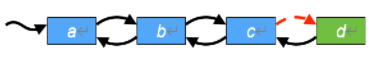
\includegraphics[width=0.3\textwidth]{1} %插入图片,[]中设置图片大小,{}中是图片文件名
    \caption{Fail to Update Relationship} %最终文档中希望显示的图片标题
    \label{linked} %用于文内引用的标签
\end{figure}

These restrictions prevent race conditions, iterator invalidation. Though, we can still use the raw pointer like in C to circumvent the restrictions, implementing cyclic data structures in Rust if we want.

% \begin{lstlisting}[language=Rust, style=boxed, caption={Doubly Linked List}]
% struct ListNode<T> {
%     data: T,
%     next: Option<Box<ListNode<T>>>,
%     prev: Option<Box<ListNode<T>>>,
% }
% impl<T> ListNode<T>{
%     fn new(data: T) -> Self {
%         ListNode{data, prev: None, next: None}
%     }
% }
% \end{lstlisting}



\end{document}